%!TEX program = xelatex
\documentclass[UTF8]{article}
\usepackage{graphicx}
\usepackage{setspace}
% \usepackage{ctex}
\usepackage{indentfirst}
\setlength{\parindent}{2em}  % 用于首行缩进

\usepackage{amsmath}
\usepackage{amsthm} % 使用定理环境
\usepackage{amssymb}

% \usepackage{geometry}
% \geometry{a4paper,scale=0.8}

\usepackage{geometry}
\geometry{a4paper,left=2.0cm,right=2.0cm,top=3.0cm,bottom=3.0cm}
\setstretch{1.5}   %  改变行间距
% \newgeometry{left = 2 cm, top= 3 cm}

\title{Summary}
\author{Dis\cdot count}
% \date{Feb 2019}

\newtheorem{thm}{\hspace{2em}Theorem}
\newtheorem{lem}{\hspace{2em}Lemma}
\newtheorem{pf}{\hspace{2em}Proof}
%  \newtheorem{def}{Definition}  doesnt work


\begin{document}

\maketitle{}

\section*{Introduction}
At first, we will introduce some preliminary knowledge about cooperative game theory as follows.
A pair $(V,c)$ is usually used to represent a cooperative game with transferable utilities, among which $V=\{1,2,\dots,v\}$ denotes a set of $v$ players and $c:2^{V}\to \mathbb{R}$ indicates the characteristic function of the game. A coalition is defined as a non-empty subset of players; while $V$ is refered to as a coalition, $S=2^{V} \setminus\{\emptyset\}$ denotes the set of all feasible coalitions. The characteristic function of the game, $c(s)$, represents the minimum coalitional cost the players in $s$ have to pay in order to cooperate together.
A cost allocation vector $\alpha=[\alpha_{1},\alpha_{2},\dots,\alpha_{v}] \in \mathbb{R}^{v}$ is required by the game to maintain cooperation in the grand coalition, and $\alpha_{k}$ is the cost assigned to players $k \in V$ to assure no individual or group of players has the incentive to deviate. For the convenience of abbreviation, we use $\alpha(s)=\sum_{k\in{s}}\alpha_{k}$ to denote the total cost assigned to the players in coalition $s$.
One of the most important concepts in cooperative game theory is core, which is a cost allocation satisfying two kinds of contraints, one is the budget balance contraint {$\alpha(V)=c(V)$} and the other is the coalitional stability constrains {$\alpha(s) \leq c(s)$}. In other words, core can be expressed as

\[
Core(V,c)= \left\{\alpha:\alpha(V)=c(V), \alpha(s)\leq c(s)\ \text{for all}\ s \in S \setminus\{V\}, \alpha \in \mathbb{R}^{v} \right\}.
\]

When the cost allocation exists, core is called non-empty. And if and only if the core is non-empty, the grand coalition of the associating cooperative game $(V,c)$ will be stable or balanced.

However, cooperative games can be unbalanced in many cases owing to the joint restrictions of the above-mentioned two kinds of constraints. To stabilize the grand coalitions in unbalanced cooperative games, researchers have already developed several effective instruments, such as subsidization, penalization and simultaneous subsidization and penalization. The
similarity of these instruments is that there exists an outside party who will take measures to stabilize the grand coalition. But the penalization will always arouse the discontent of players in coalitions, it's promising to find a new instrment to replace the penalization, we call it taxation.
The significant idea of this instrument is that we can erase the role of the third party by collecting taxation as subsidy of the corresponding coalitions.
That being said, the players of the games can stabilize themselves without the third party.


To make the project concrete, we will apply the cooperative theory on the machine schedule problem to show our ideas.


Then we will illustrate the taxation instrument with a simple example of an IPU (Identical Parallel machine scheduling of Unweighted jobs) game as follows.

\section*{Example}

There is a IPU game which contains four players, whose processing times on the identical parallel machine are $t_1=2,t_2=3,t_3=4,t_4=5$ respectively. Each machine setup cost is $t_0=9.5$, and $c(s)$ is the minimum total completion time of jobs in coalition $s$ plus the machine setup cost.

In this example, the grand coalition has a minimum cost of 38, and the optimum number of machine is 2.
It's easy to check that this example is unbalanced and calculate the subsidy which equals $ c(V) - \alpha(V) = 0.75$.

When the setup cost increases from 9.5 to 13, that is, the taxation increases from 0 to 3.5,
the number of machine will decrease from 2 to 1, accordingly.

Although this case is easily understood, it demonstrate the concept of taxation we have strong interests in. Then we will define the corresponding model to further elaborate on this concept.

\section*{Definition 1.}

A cooperative TU game $(V,c)$ is called an IPU game if it satisfies the following formulations.

\[
\begin{aligned}
c(s,m(s,P)) = & {\min} \sum_{k\in V}\sum_{j\in O} {c_{kj} x_{kj}} + { Pm} \\
{s.t.}\quad & \sum_{j \in O} x_{kj}-y_k^s=0, \forall k \in V, \\
& \sum_{k\in V} x_{kj} \leq m(s),\forall j \in O,  \\
& \sum_{k\in s} x_{k1}=m(s), \\
& x_{kj} \in \{0,1\} , \forall k \in V, \forall j \in O,\\
& y_k^s=1, k \in s, y_k^s=0, k \notin s.
\end{aligned}
\]
Among these formulations, $P$ and $m$ denote the price and the number of using machines, respectively.
Now we've already extended the number of players to a more complex case, that is, the number of players is set to $n$.
Let $N=\{1,2,\ldots,n\}$ be a set of n players. The number of machines is $m$ and the setup cost is $t_0$.
For convenience of expression, we set the processing times $t_i, i\in N$ satisfy $t_1<t_2<\cdots<t_n$.

Then we need to define a function, that is, subsidy-price function denoted by $\omega(P)$:
\[
  {\omega(P)}=\mathop{\min}_{\alpha}\{c(V,m(V,P))-\alpha(V): \alpha(s)\leq c(s,m(s,P))
 \forall s \in S, \alpha\in\mathbb{R}^{v}\}.
\]

By obtaining its dual:
\begin{equation}\label{dual}
 {\omega^*(P)}=\mathop{\max}_{\rho} \{c_0(V)+m(V)P+\sum_{s\in S\setminus\{V\}}-\rho_s[c_0(s)+m(s)P]:
 \sum_{s\in S\setminus\{V\}:k\in s}\rho_s=1,\forall k \in V,\rho_s\geq 0,\forall s \in S \setminus{V}\}
\end{equation}

we can establish Theorem 1 below, showing the property of the function.

\begin{thm}\label{thm1}

$\omega(P)$ is piecewise linear, and convex in price P when $m(V)$ is a fixed integer.
\end{thm}


In this situation, the interval size of setup cost can be calculated when $t_i$ is known. And we can obtain that under what circumstances the machine number will change. We set the different intervals where the number of machines remain unchanged as $I_i$ respectively. The extreme points of these intervals are recorded as $P_i$ respectively, which represents the price when the number of using machine changes from $i$ to $i-1$. Specially, $P_1$ denotes the extreme point of the whole interval, which is the value of price or setup cost when using one machine and subsidy equals zero.

Note that the costs of all the exponential coalitions can be easily calculated by the SPT rules, we have Lemma \ref{lem1}.

\begin{lem}\label{lem1}

The value at the extreme points of the sub-intervals $I_i$ can be calculated with processing times $t_i$ by comparing the costs of the grand coalitions where all the players use two adjacent numbers of machines.
\end{lem}

According to the above lemma \ref{lem1}, we can obtain all the extreme points of the sub-intervals, i.e. , the number of using machines decreases by one when the price or setup cost equals $P_i$.


\begin{thm}\label{thm2}

According to the foregoing description, we have the equation $S_{1}=S_{2}+\cdots+S_{n}=\sum_{i=2}^n S_i$.

\end{thm}

With Theorem \ref{thm2}, we obtain all the breakpoints during the interval of the price where the machine number changes and the subsidy is $0$. Then we'll focus on the specific property of subsidy.

\begin{thm}\label{thm3}

The subsidy is always zero when m is larger than $\frac{n}{2}$. In other words, when the numbers of machine is larger than half of players, the grand coalition don't need any subsidy from the externality.

\end{thm}

\begin{thm}\label{thm4}

When the number of machines used is 1, the range of slopes of the line segments in the interval is $\left( -1 , -\frac{1}{n-1} \right]$, and the number of breakpoints is $ O(v^2) $.
\end{thm}

Until here, we described the main property of the whole figure.
And a diagram of the number of machines and subsidy on setup cost, with its essential features being showed below.

\begin{figure}[h]%%图
	\centering  %插入的图片居中表示
	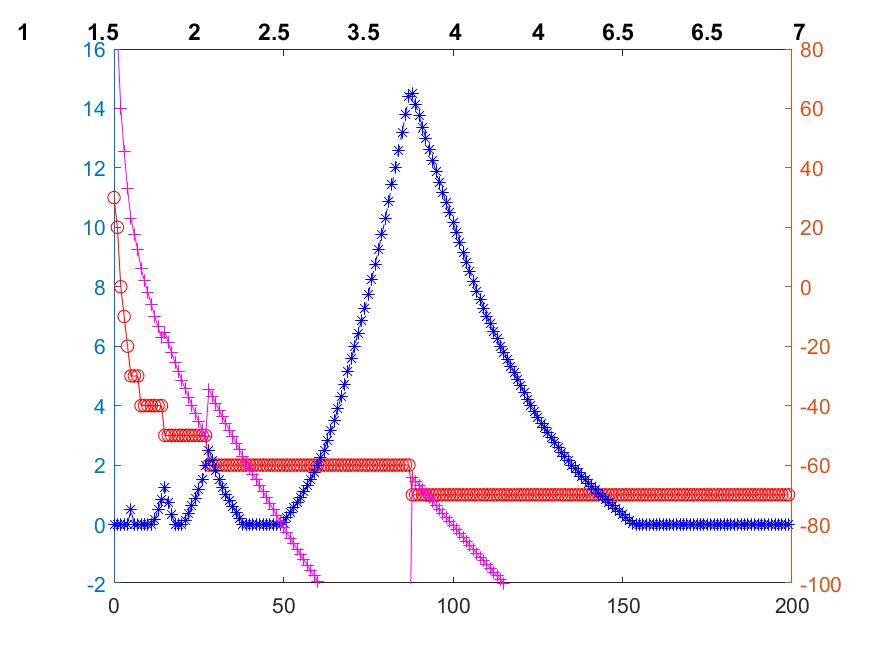
\includegraphics[width=0.8\linewidth]{Figures/Image30}  %插入的图,包括JPG,PNG,PDF,EPS等,放在源文件目录下
	\caption{The number of machines and subsidy on setup cost.}  %图片的名称
	\label{fig:Image11}   %标签,用作引用
\end{figure}

The processing times of all players with the arrangement from small to large are listed on the top of this figure.
The red and blue lines stand for the machine number and subsidy, respectively.
The horizontal ordinate represents the price or setup cost.
The left ordinate represents the value of machine number,while the right represents the value of subsidy.

As the coalitional stability constrains showed above, the exponential inequality constraints are so tricky that we must figure out a method to simplify these constraints to obtain the optimal results. Fortunately for us, we find the Theorem \ref{thm5}.


\begin{thm}\label{thm5}

When changing the price $P$, the effective inequalities correspond to the coalitions using only one machine.
\end{thm}

By establishing the Theorem 5, we can design the specific algorithm to eliminate the redundant inequalitie, which will save us the trouble of solving $c(s)$ and speed up the solution.

\begin{thm}\label{thm6}
The IPU game can be solved in polynomial time.(Remaining to be proved)
\end{thm}

Now that we've already solved the IPU game, we will try to extend the core concept to a more general case. So we need to define a new game as follow.

\section*{Definition 2}

A cooperative TU game $(V,c)$ is a PIM(Price Integer Minimization) game if there exist:

\begin{itemize}
	\item positive integers e, v, t, P and m;
	\item integer vectors $ x \in \mathbb{Z}^{t \times 1} $and $ \tilde{\alpha} \in \mathbb{Z}^{1 \times t} $;
	\item left hand side matrix  $A \in \mathbb{R} ^{e \times t};$
	\item right hand side matrix $B \in \mathbb{R} ^ {e \times v};$
	\item a right hand side vector $D \in \mathbb{Z} ^ {e};$
	\item an objective function vector
	$c \in \mathbb{Z}^{1 \times t};$
	\item an incidence vector $y^s \in \{0,1\}^v$ with $y^s_k = 1$ if $k \in s$ and $y^s_k = 0 $ otherwise, $\forall k \in V$,

\end{itemize}

such that the characteristic function $c(s)$ equals the optimal objective value of the following integer linear program:

\[
c(s,m(s,P))= \mathop{\min}_{x} \{ cx+Pm: Ax \geq By^s+D, \tilde{\alpha}x \leq m, x \in \mathbb{Z}^{t \times 1} \}
\]

Note that the object function is not easy to analyze due to the joint effct of $cx$ and $Pm$, we need to divide the function into two parts for a further discussion.

With this idea, we divide $c(s,m(s,P))$ as $c_0(s,m(s))+Pm $. Via analysis and study, we find some properties about $c_0(s,m(s)) $ which we call primary function later.

The primary function must be supermodular, then we can get the positive price or setup cost when the number of facilities changes. This corresponds to the following two lemmas.

\begin{lem}\label{lem2}
\[
c_0 (s,m) - c_0 (s,m+1) > 0 \Leftrightarrow P_i > 0
\]
\end{lem}

\begin{lem}\label{lem3}
\[
\begin{aligned}
&c_0 (s,m) - c_0 (s,m+1) < c_0 (s,m-1) - c_0 (s,m) \\
& \Leftrightarrow \quad P_i < P_{i-1} , i=3,4,\cdots,n
\end{aligned}
\]
\end{lem}


Once the primary function must be supermodular, we can specify this property in the following two aspects.
One is the concavity about the number of facilities,
the other is the nature about the number of players($s_1 \subset s_2$).
They correspond to the following two formulas:

\begin{equation}\label{concavity_f}
c_0(s_1,m(s_1)-1)-c_0(s_1,m(s_1)) \geq
  c_0(s_1,m(s_1))-c_0(s_1,m(s_1)+1)
\end{equation}

and

\begin{equation}\label{property_p}
	c_0(s_1,m(s_1)-1)-c_0(s_1,m(s_1)) \leq
	  c_0(s_2,m(s_1)-1)-c_0(s_2,m(s_1))
\end{equation}
, respectively.

Then we can develop the Theorem \ref{thm7}.

\begin{thm}\label{thm7}

When coalitions $s_1,s_2$ satisfy $s_1 \subset s_2$, the corresponding number of using facilities $ m_{s_1}, m_{s_2}$ have $m_{s_1} \leq m_{s_2}$, if the primary function satisfies  (\ref{concavity_f}) and (\ref{property_p}).
\end{thm}


\begin{pf}[Lemma 1]
  In fact, according to the SPT rule, a fixed number of using machines for the given grand coalition corresponds to the only deterministic sort order working on the machines, i.e. the deterministic cost. Therefore, by comparing the cost of the number of adjacent machines $(k, k + 1)$ used by the grand coalition, the corresponding setup cost or the price $P_i$ can be obtained.
  \qed
\end{pf}


\begin{pf}[Theorem 2]

For convenience of expression, we set the setup cost as $S_{1},S_{2}, \dots ,S_{n}$ at interval points while the number of machine changes.
And $S_{i}$ denotes the setup cost when the machine number changes from $i$ to $i-1$, especially, $S_{1}$ denotes the least setup cost when machine number is $1$ and the corresponding subsidy is $0$.
We just need to prove the following equality

\begin{displaymath}
  S_{1}=S_{2}+\cdots+S_{n}=\sum_{i=2}^n S_i.
\end{displaymath}

Notice that

\begin{displaymath}
  (n-1) \sum_{s \in S \setminus\{V\} } \rho_s \geq
  \sum_{k\in V}\sum_{s \in S \setminus\{V\}:k \in s} \rho_s = n.
\end{displaymath}

The left side of the inequality means for every $\rho_s$ can appear at most $(n-1)$ times, so we should know that if and only if for every $\rho_s > 0$ appears $n-1$ times the quality holds.That is to say, the coalitions which contains $n-1$ players are all maximally unsatisfied coalitions. Then we have $n \choose n-1$ equalities.
\[
\begin{cases}
 \alpha_1+\alpha_2+ \cdots+\alpha_{n-1} & = x_1 \\
 \alpha_1+\alpha_3+ \cdots+\alpha_n & = x_2 \\
 \quad   \vdots        &\vdots\\
 \alpha_2+\alpha_3+ \cdots+\alpha_n & = x_n.
\end{cases}
\]

Add these $n$ equations together, and we can get

\begin{equation*}
  (n-1)(\alpha_1+\alpha_2+ \cdots+\alpha_n)=\sum_{i=1}^{n}x_i
\end{equation*}

As we know, $x_1,x_2,\dots,x_n$ can be expressed as follows:

\[
\begin{cases}
x_1 = S_0 + (n-1)t_1 + (n-2)t_2 + &\cdots + t_{n-1} \\
x_2 = S_0 + (n-1)t_1 + (n-2)t_3 + &\cdots + t_{n-1} \\
\quad   \vdots        &\vdots\\
x_n = S_0 + (n-1)t_2 + (n-2)t_3 + &\cdots + t_{n}
\end{cases}
\]

According to SPT rule, we can obtain the equality
$c(V)=\alpha_1+\alpha_2+\cdots+\alpha_n=S_0+nt_1+(n-1)t_2+\dots+t_n$.
By replacing $x_1,x_2,\dots,x_n$ together with the expression of $c(V)$, we can get a equality only with $S_0,x_1,x_2,\dots,x_n$.

Finally, we can obtain $S_0 = \sum_{k=1}^n (n-k)t_k$.
\qed
\end{pf}


\begin{pf}[Theorem 1]

By deriving from $\omega^* (P)$ (\ref{dual}),it can be seen that the SPF $\omega(P)$ is in fact the point-wise maximum of a set of straight lines, $c_0(V)+m(V)P+\sum_{s\in S\setminus\{V\}}-\rho_s[c_0(s)+m(s)P]$, each with a slope of $m(V)+\sum_{s\in S\setminus\{V\}} −\rho_s m(s)$, for $\rho$ in $\{\rho :\sum_{s\in S\setminus \{V\}:k\in s} \rho_s=1  \text{for all }  k\in V, \text{and } \rho_s \geq 0 \text{for all } s\in S\setminus \{V\} \}$.
Meanwhile, it's easy to see that $m(s)$ does not increase as P increases. Thus, we can claim that the SPF $\omega(P)$ is a convex function in P when $m(V)$ is a fixed integer.

Notice that the existence of $m(V)$ does not affect the property of the numbers of the breakpoints.
% 注意这里还需要说明 [0,P*]
To show that the SPF $\omega^* (P)$ is a piecewise linear function with a finite number of breakpoints, consider the feasible region of LP (\ref{dual}) for $\omega^* (P)$ without the part of $m(V)$ that is written as $\acute{\omega} (P)$, which is a convex polyhedron, denoted by $\hat{R}$. It can be seen that $\hat{R}$ has a finite number of extreme points, and is independent of P. For any given $P \in [0,P^*]$, by LP (\ref{dual}) we know that there must exist an extreme point $\rho$ of $\hat{R}$ such that $\acute{\omega} (P)$ equals
$c_0(V)+m(V)P+\sum_{s\in S\setminus\{V\}}-\rho_s[c_0(s)+m(s)P]$
and that the derivative of $\acute{\omega} (P)$ at P equals $\sum_{s\in S\setminus\{V\}} −\rho_s m(s)$. Thus, the derivative of $\acute{\omega} (P)$ for $P \in [0,P^*]$ can have only a finite number of possible values. Moreover, due to the convexity of $\acute{\omega} (P)$, the derivative of $\acute{\omega} (P)$ is non-decreasing in P. Hence, the derivative of $\acute{\omega} (P)$ can change for only a finite number of times when P increases from 0 to $P^*$. Therefore, $\omega^* (P)$ is a piecewise linear function with a finite number of breakpoints.
\qed
\end{pf}




\begin{pf}[Theorem 3.]

	注意这一条定理只针对于 机器调度 根本原因在于 排序性(一个接一个  而不会存在 一台一个一台三个)

\end{pf}


\begin{pf}[Theorem 4.]

需要仿照 原来证明 注意断点的证明较复杂


\end{pf}



\begin{pf}[Theorem 5.]

只	需要证明 不等式分解 次序即可

\end{pf}

\begin{pf}[Theorem 6.]

Remaining

\end{pf}

\begin{pf}[Lemma 2.]

注意这个证明  只与c_0(s) 有关

\end{pf}


\end{document}
